\ifx\wholebook\relax \else
% ------------------------

\documentclass[b5paper]{article}
\usepackage[nomarginpar
  %, margin=.5in
]{geometry}

\addtolength{\oddsidemargin}{-0.05in}
\addtolength{\evensidemargin}{-0.05in}
\addtolength{\textwidth}{0.1in}

\usepackage[en]{../../../prelude}

\setcounter{page}{1}

\begin{document}

\title{AVL tree - proofs and the delete algorithm}

\author{Xinyu LIU
\thanks{{\bfseries Xinyu LIU} \newline
  Email: liuxinyu95@gmail.com \newline}
  }

\maketitle
\fi

\markboth{AVL tree - proofs and the delete algorithm}{Elementary Algorithms}

\ifx\wholebook\relax
\chapter{AVL tree - proofs and the delete algorithm}
\numberwithin{Exercise}{chapter}
\fi

\section{Height increment}

When insert an element, the increment of the height can be deduced
into 4 cases:

\be
\begin{array}{rcl}
  \Delta H & = & |T'| - |T| \\
           & = & 1 + max(|r'|, |l'|) - (1 + max(|r|, |l|)) \\
           & = & max(|r'|, |l'|) - max(|r|, |l|) \\
           & = & \begin{cases}
\delta \geq 0, \delta' \geq 0: & \Delta r \\
\delta \leq 0, \delta' \geq 0: & \delta + \Delta r \\
\delta \geq 0, \delta' \leq 0: & \Delta l - \delta \\
otherwise: & \Delta l
\end{cases}
\end{array}
\ee

\begin{proof}
When insert, the height can not increase both on left and right. We can explain the 4 cases from the balance factor definition, that it equals to the difference of the right and left sub-trees:

\begin{itemize}
\item If $\delta \geq 0$ and $\delta' \geq 0$, it means the height
of the right sub-tree is not less than the left sub-tree before and after insertion. In this case, the height increment is only `contributed' from the right, which is $\Delta r$.

\item If $\delta \leq 0$, it means the height of left sub-tree is not less than the right before. Since $\delta' \geq 0$ after insert, we know the height of right sub-tree increases, and the left side keeps same ($|l'|=|l|$). The height increment is:

\[
\begin{array}{rll}
\Delta H & = max(|r'|, |l'|) - max (|r|, |l|) & \{\delta \leq 0\ \text{and}\ \delta' \geq 0 \}\\
         & = |r'|-|l| & \{|l|=|l'|\}\\
         & = |r|+\Delta r - |l| & \\
         & = \delta + \Delta r & \\
\end{array}
\]

\item If $\delta \geq 0$ and $\delta' \leq 0$, similar to the above case, we have the following:

\[
\begin{array}{rll}
\Delta H & = max(|r'|, |l'|) - max (|r|, |l|) & \{\delta \geq 0\ \text{and}\ \delta' \leq 0 \}\\
         & = |l'|-|r| & \\
         & = |l| + \Delta l - |r| & \\
         & = \Delta l - \delta & \\
\end{array}
\]

\item Otherwise, $\delta$ and $\delta'$ are not bigger than zero. It means the height of the left sub-tree is always greater than or equal to the right. The height increment is only `contributed' from the left, which is $\Delta l$.
\end{itemize}
\end{proof}

\section{Balance adjustment after insert}

The balance factors are $\pm 2$ in the 4 cases shown in figure \ref{fig:avl-insert-fix-appendix}. After fixing, $\delta(y)$ resumes
to 0. The height of left and right sub-trees are equal.

\begin{figure}[htbp]
  \centering
  \includegraphics[scale=0.4]{../../../datastruct/tree/AVL-tree/img/avl-insert-fix.png}
  \caption{Fix 4 cases to the same structure}
  \label{fig:avl-insert-fix-appendix}
\end{figure}

The four cases are left-left, right-right, right-left, and left-right. Let the balance factors before fixing be $\delta(x), \delta(y)$, and $\delta(z)$, after fixing, they change to $\delta'(x), \delta'(y)$, and $\delta'(z)$ respectively. We next prove that, $\delta(y)=0$ for all 4 cases after fixing, and give the result of $\delta'(x)$ and $\delta'(z)$.

\subsubsection*{Left-left}

The sub-tree $x$ keeps unchanged, hence $\delta'(x) = \delta(x)$. As $\delta(y) = -1$ and $\delta(z) = -2$, we have:

\be
  \begin{array}{rcl}
  \delta(y) = |c| - |x| = -1 & \Rightarrow & |c| = |x| - 1 \\
  \delta(z) = |d| - |y| = -2 & \Rightarrow & |d| = |y| - 2 \\
  \end{array}
  \label{eq:ll-cd}
\ee

After fixing:

\be
  \begin{array}{rcll}
  \delta'(z) & = & |d| - |c| & \{ from (\ref{eq:ll-cd}) \}\\
             & = & |y| - 2 - (|x| - 1) & \\
             & = & |y| - |x| - 1 & \{  x \text{ is sub-tree of } y \Rightarrow |y|-|x| = 1\} \\
             & = & 0 & \\
  \end{array}
  \label{eq:ll-delta-z}
\ee

For $\delta'(y)$, we have the following:

\be
  \begin{array}{rcll}
  \delta'(y) & = & |z| - |x| & \\
             & = & 1 + max(|c|, |d|) - |x| & \{ \text{by (\ref{eq:ll-delta-z}), } |c| = |d|\} \\
             & = & 1 + |c| - |x| & \{ \text{by (\ref{eq:ll-cd})}\} \\
             & = & 1 + |x| - 1 - |x| & \\
             & = & 0 & \\
  \end{array}
\ee

Summarize the above, the balance factors change to the following in left-left case:

\be
  \begin{array}{l}
  \delta'(x) = \delta(x) \\
  \delta'(y) = 0 \\
  \delta'(z) = 0
  \end{array}
\ee

\subsubsection*{Right-right}

The right-right case is symmetric to left-left:

\be
  \begin{array}{l}
  \delta'(x) = 0 \\
  \delta'(y) = 0 \\
  \delta'(z) = \delta(z)
  \end{array}
  \label{eq:rr-result}
\ee

\subsubsection*{Right-left}

Consider $\delta'(x)$, after fixing, it is:

\be
  \delta'(x) = |b| - |a|
  \label{eq:rl-dx}
\ee

Before fixing, the height of $z$ can be obtained as:

\be
  \begin{array}{rll}
  |z| & = 1 + max(|y|, |d|) &  \{ \delta(z) = -1 \Rightarrow |y| > |d|\} \\
      & = 1 + |y| & \\
      & = 2 + max(|b|, |c|)
  \end{array}
  \label{eq:rl-z}
\ee

Since $\delta(x) = 2$, we have:

\be
  \begin{array}{rll}
  \delta(x) = 2 & \Rightarrow |z| - |a| = 2 & \{ \text{by (\ref{eq:rl-z})} \}\\
                & \Rightarrow 2 + max(|b|, |c|) - |a| = 2 & \\
                & \Rightarrow max(|b|, |c|) - |a| = 0 &
  \end{array}
  \label{eq:rl-ca}
\ee

If $\delta(y) = 1$, then $|c| - |b| = 1$. We have:

\be
  max(|b|, |c|) = |c| = |b| + 1
\ee

Take this into (\ref{eq:rl-ca}) gives:

\be
  \begin{array}{ll}
  |b| + 1 - |a| = 0 \Rightarrow |b|-|a|= -1 & \{ \text{by (\ref{eq:rl-dx}) } \} \\
  \Rightarrow \delta'(x) = -1 &
  \end{array}
\ee

If $\delta(y) \neq 1$, then $max(|b|, |c|) = |b|$. Take this into (\ref{eq:rl-ca}) gives:

\be
  \begin{array}{ll}
  |b| - |a| = 0  & \{ \text{by (\ref{eq:rl-dx})} \} \\
  \Rightarrow \delta'(x) = 0 &
  \end{array}
\ee

Summarize the 2 cases, we obtained the result of $\delta'(x)$ in $\delta(y)$ as the following:

\be
\delta'(x) = \begin{cases}
  \delta(y) = 1: & -1 \\
  otherwise: & 0 \\
\end{cases} \\
\label{eq:rl-dx-dy}
\ee

For $\delta'(z)$, from the definition, it equals to:

\be
  \begin{array}{rcll}
    \delta'(z) & = & |d| - |c| & \{ \delta(z) = -1 = |d| - |y| \} \\
               & = & |y| - |c| - 1 & \{ |y| = 1 + max(|b|, |c|) \} \\
               & = & max(|b|, |c|) - |c| \\
  \end{array}
  \label{eq:rl-dz}
\ee

If $\delta(y) = -1$, then $|c| - |b| = -1$, $max(|b|, |c|) = |b| = |c| + 1$. Take this into (\ref{eq:rl-dz}), we have $\delta'(z) = 1$.

If $\delta(y) \neq -1$, then $max(|b|, |c|) = |c|$. We have $\delta'(z) = 0$.

Combined these two cases, we obtained the result of $\delta'(z)$ in $\delta(y)$ as below:

\be
  \delta'(z) = \begin{cases}
    \delta(y) = -1: & 1 \\
    otherwise: & 0 \\
    \end{cases} \\
  \label{eq:rl-dz-dy}
\ee

Finally, for $\delta'(y)$, we deduce it like below:

\be
  \begin{array}{rl}
  \delta'(y) & = |z| - |x| \\
             & = max(|c|, |d|) - max(|a|, |b|)
  \end{array}
  \label{eq:rl-dy}
\ee

There are three cases:

\begin{itemize}
\item If $\delta(y)=0$, then $|b|=|c|$. According to (\ref{eq:rl-dx-dy}) and (\ref{eq:rl-dz-dy}), we have $\delta'(x)=0 \Rightarrow |a| = |b|$, and $\delta'(z)=0 \Rightarrow |c|=|d|$. These lead to $\delta'(y)=0$.

\item If $\delta(y)=1$, from (\ref{eq:rl-dz-dy}), we have $\delta'(z)=0 \Rightarrow |c| = |d|$.
\[
  \begin{array}{rcll}
  \delta'(y) & = & max(|c|, |d|) - max(|a|, |b|) & \{|c|=|d|\} \\
             & = & |c| - max(|a|, |b|) & \{\text{from (\ref{eq:rl-dx-dy}): $\delta'(x)=-1 \Rightarrow |b|-|a|=-1$} \} \\
             & = & |c| - (|b| + 1) & \{ \delta(y) = 1 \Rightarrow |c|-|b|=1\} \\
             & = & 0 \\
  \end{array}
\]

\item If $\delta(y)=-1$, from (\ref{eq:rl-dx-dy}), we have $\delta'(x)=0 \Rightarrow |a|=|b|$.
\[
  \begin{array}{rcll}
  \delta'(y) & = & max(|c|, |d|) - max(|a|, |b|) & \{|a|=|b|\} \\
             & = & max(|c|, |d|) - |b| & \{ \text{from (\ref{eq:rl-dz-dy}): $|d|-|c|=1$} \} \\
             & = & |c| + 1 - |b| & \{  \delta(y) = -1 \Rightarrow |c|-|b|=-1\} \\
             & = & 0 \\
  \end{array}
\]

\end{itemize}

All three cases lead to the same result $\delta'(y)=0$. Summarize all above, we get the updated balance factors after fixing as below:

\be
  \begin{array}{l}
  \delta'(x) = \begin{cases}
    \delta(y) = 1: & -1 \\
    otherwise: & 0 \\
    \end{cases} \\
  \delta'(y) = 0 \\
  \delta'(z) = \begin{cases}
    \delta(y) = -1: & 1 \\
    otherwise: & 0 \\
    \end{cases} \\
  \end{array}
  \label{eq:rl-result}
\ee

\subsubsection*{Left-right}

Left-right is symmetric to the right-left case. With similar method, we can obtain the new balance factors that is identical to (\ref{eq:rl-result}).

\section{Delete algorithm}

Deletion may reduce the height of the sub-tree. If the balance factor exceeds the range of $[-1, 1]$, then we need fixing.

\subsection{Functional delete}

We can reuse most of the deletion algorithm for BST, then check the balance factor
and perform fixing. Similiar to the insertion algorithm, the result after deletion
is a pair $(T', \Delta H)$, where $T'$ is the new tree and $\Delta H$ is the decrement
of the height. Let function $first(pair)$ return the first component in a pair.
We define the deletion algorithm as below.

\be
delete(T, k) = first(del(T, k))
\ee

where

\be
del(T, k) = \left \{
  \begin{array}
  {r@{\quad:\quad}l}
  (\phi, 0) & T = \phi \\
  tree(del(T_l, k), k', (T_r, 0), \Delta) & k < k' \\
  tree((T_l, 0), k', del(T_r, k), \Delta) & k > k' \\
  (T_r, -1) & k = k', T_l = \phi \\
  (T_l, -1) & k = k', T_r = \phi \\
  tree((T_l, 0), k'', del(T_r, k''), \Delta) & otherwise, k'' = min(T_r)
  \end{array}
\right.
\label{eq:avl-del}
\ee

If the tree is empty, the result is empty as well; Otherwise, we compare the
key with the value to be delete and recursively lookup and perform delete
along the sub trees. If the node to be delete has only one child, we cut
that node off. Otherwise, we use the minimum value in the right sub tree
to replace the key, and cut the minimum node off.

We can reuse the $tree()$ function, as well as the result for $\Delta H$.
But different from insertion, there are extra two cases can violate AVL
properties, thus need fixing.

\begin{figure}[htbp]
  \centering
  \subcaptionbox{Fix AVL violation after deletion. case A}{
    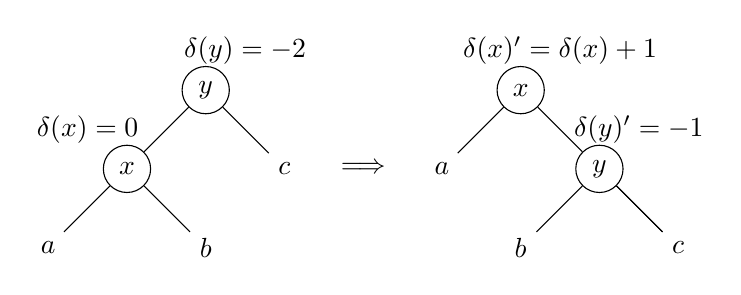
\begin{tikzpicture}[scale=1,
        trnode/.style={circle, draw, inner sep= 0pt, minimum size = .6cm}
      ]
      % left side
      \node[trnode] at (0, 0) (y) {$y$};
      \node[trnode] at (-1, -1) (x) {$x$};
      \draw (1, -1) node (c) {$c$};
      \draw (-2, -2) node (a) {$a$};
      \draw (0, -2) node (b) {$b$};
      % edges
      \draw (y) -- (x) -- (a);
      \draw (y) -- (c);
      \draw (x) -- (b);
      % labels
      \draw (0.5, 0.5) node{$\delta(y) = -2$};
      \draw (-1.5, -0.5) node{$\delta(x) = 0$};

      % right side
      \node[trnode] at (4, 0) (x1) {$x$};
      \draw (3, -1) node (a1) {$a$};
      \node[trnode] at (5, -1) (y1) {$y$};
      \draw (4, -2) node (b1) {$b$};
      \draw (6, -2) node (c1) {$c$};
      % edges
      \draw (x1) -- (y1) -- (c1);
      \draw (x1) -- (a1);
      \draw (y1) -- (b1);
      \draw (y1) -- (c1);
      % labels
      \draw (4.5, 0.5) node{$\delta(x)' = \delta(x) + 1$};
      \draw (5.5, -0.5) node{$\delta(y)' = -1$};

      \draw (2, -1) node{$\Longrightarrow$};
  \end{tikzpicture}} \\
  \subcaptionbox{Fix AVL violation after deletion. case B}{
    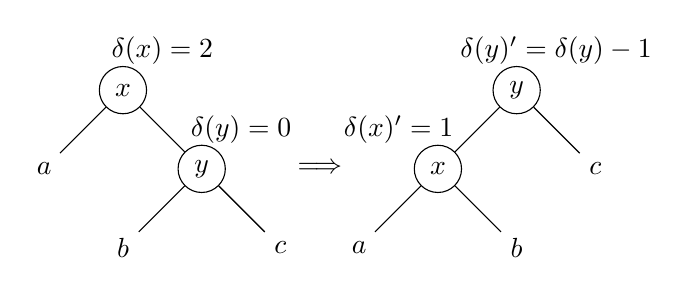
\begin{tikzpicture}[scale=1,
        trnode/.style={circle, draw, inner sep= 0pt, minimum size = .6cm}
      ]
      % left side
      \node[trnode] at (0, 0) (x) {$x$};
      \draw (-1, -1) node (a) {$a$};
      \node[trnode] at (1, -1) (y) {$y$};
      \draw (0, -2) node (b) {$b$};
      \draw (2, -2) node (c) {$c$};
      % edges
      \draw (x) -- (y) -- (c);
      \draw (x) -- (a);
      \draw (y) -- (b);
      \draw (y) -- (c);
      % labels
      \draw (0.5, 0.5) node{$\delta(x) = 2$};
      \draw (1.5, -0.5) node{$\delta(y) = 0$};

      % right side
      \node[trnode] at (5, 0) (y1) {$y$};
      \node[trnode] at (4, -1) (x1) {$x$};
      \draw (6, -1) node (c1) {$c$};
      \draw (3, -2) node (a1) {$a$};
      \draw (5, -2) node (b1) {$b$};
      % edges
      \draw (y1) -- (x1) -- (a1);
      \draw (y1) -- (c1);
      \draw (x1) -- (b1);
      % labels
      \draw (5.5, 0.5) node{$\delta(y)' = \delta(y) - 1$};
      \draw (3.5, -0.5) node{$\delta(x)' = 1$};


      \draw (2.5, -1) node{$\Longrightarrow$};
  \end{tikzpicture}}
  \caption{AVL tree fixing for delete} \label{fig:avl-del-fixing}
\end{figure}

As shown in figure \ref{fig:avl-del-fixing}, both cases can be fixed by a tree rotation. It can be essentailly catpured by pattern matching to the tree structure.

\be
balance(T, \Delta H) = \left \{
  \begin{array}
  {r@{\quad:\quad}l}
  ... \\
  (A, x, (B, y, C, -1), \delta(x) + 1, \Delta H) & T = ((A, x, B \delta(x)), y, C, -2, \Delta H) \\
  ((A, x, B 1), y, C, \delta(y) - 1, \Delta H) & T = (A, x, (B, y, C \delta(y)), 2, \Delta H) \\
  ...
  \end{array}
\right.
\ee

Below is the example program in Haskell

\lstset{language=Haskell}
\begin{lstlisting}
delete::(Ord a) => AVLTree a -> a -> AVLTree a
delete t x = fst $ del t x where
  -- result is a pair (t, d), t: tree, d: decrement in height
  del Empty _ = (Empty, 0)
  del (Br l k r d) x
    | x < k = node (del l x) k (r, 0) d
    | x > k = node (l, 0) k (del r x) d
    -- x == k, delete this node
    | isEmpty l = (r, -1)
    | isEmpty r = (l, -1)
    | otherwise = node (l, 0) k' (del r k') d where k' = min r
\end{lstlisting}

Where the auxiliary function \texttt{min} are implemented similiar to the binary
search tree, it traverses along the left sub tree till the end. Function \texttt{isEmpty} test if a tree is empty.

\begin{lstlisting}
isEmpty Empty = True
isEmpty _ = False

min :: AVLTree a -> a
min (Br Empty x _ _) = x
min (Br l _ _ _) = min l
\end{lstlisting}

After adding the extra two cases for fixing, there are total 7 cases in the \texttt{balance} function.

\begin{lstlisting}
balance :: (AVLTree a, Int) -> (AVLTree a, Int)
balance (Br (Br (Br a x b dx) y c (-1)) z d (-2), dH) =
        (Br (Br a x b dx) y (Br c z d 0) 0, dH-1)
balance (Br a x (Br b y (Br c z d dz)    1)    2, dH) =
        (Br (Br a x b 0) y (Br c z d dz) 0, dH-1)
balance (Br (Br a x (Br b y c dy)    1) z d (-2), dH) =
        (Br (Br a x b dx') y (Br c z d dz') 0, dH-1) where
    dx' = if dy ==  1 then -1 else 0
    dz' = if dy == -1 then  1 else 0
balance (Br a x (Br (Br b y c dy) z d (-1))    2, dH) =
        (Br (Br a x b dx') y (Br c z d dz') 0, dH-1) where
    dx' = if dy ==  1 then -1 else 0
    dz' = if dy == -1 then  1 else 0
-- Delete specific fixing
balance (Br (Br a x b dx) y c (-2), dH) = (Br a x (Br b y c (-1)) (dx+1), dH)
balance (Br a x (Br b y c dy)    2, dH) = (Br (Br a x b    1) y c (dy-1), dH)
balance (t, d) = (t, d)
\end{lstlisting}

\subsection{Imperative deletion}

Imperative deletion algorithm uses tree rotation to resume the balance of the tree.
There are more cases need to handle. We firstly apply the binary search tree deletion
process, then fix the balance if it violates the AVL properties due to the sub tree
height shrink. The main deletion algorithm is given as the following.

\begin{algorithmic}[1]
\Function{Delete}{$T, x$}
  \If{$x = $ NIL}
    \State \Return $T$
  \EndIf
  \State $p \gets$ \Call{Parent}{$x$}
  \If{\Call{Left}{$x$} = NIL}
    \State $y \gets $ \Call{Right}{$x$}
    \State replace $x$ with $y$
  \ElsIf{\Call{Right}{$x$} = NIL}
    \State $y \gets $ \Call{Left}{$x$}
    \State replace $x$ with $y$
  \Else
    \State $z \gets$ \textproc{Min}(\Call{Right}{$x$})
    \State copy key and satellite date from $z$ to $x$
    \State $p \gets$ \Call{Parent}{$z$}
    \State $y \gets$ \Call{Right}{$z$}
    \State replace $z$ with $y$
  \EndIf
  \State \Return \Call{AVL-Delete-Fix}{$T, p, y$}
\EndFunction
\end{algorithmic}

If the node subject to delete is empty, the tree doesn't change. In normal case,
we record the parent of that node as $p$. If either of sub tree is empty, we
cut off the node, and replace it with the other sub tree. Otherwise, we locate
the node contains the minimum key from the right sub tree as $z$, copy the key and the
satellite data to $x$, then cut $z$ off. Finally, we call the fixing function
and pass the root, the parent, and the node replaces the removed one as parameters.

Denote the balance factor of the parent node as $\delta(p)$, by checking the new value
$\delta(p)'$, there are three different cases.

\begin{itemize}
\item Case 1, $|\delta(p)| = 0$, $|\delta(p)'| = 1$. It means, after deletion,
although one sub tree height shrinks, the parent node still satisfies the AVL
property. The algorithm terminates as the tree is still balanced;
\item Case 2, $|\delta(p)| = 1$, $|\delta(p)'| = 0$. It means before the deletion,
the height difference between the two sub trees are 1; while after deletion, the
sub tree with greater height shrinks by 1, thus the heights are same now. As the
result, the height of the parent tree also decrease by 1. We need go on the
bottom-up updating along the parent link towards the root;
\item Case 3, $|\delta(p)| = 1$, $|\delta(p)'| = 2$. It means the tree after deletion
violates the AVL property, we need fix it by tree rotation.
\end{itemize}

For case 3, most of fixing operations are similar to to insertion fixing. However,
we need add two extra sub cases to cover the situations illustrated in figure
\ref{fig:avl-del-fixing}. The fixing algorithm is given as the following.

\begin{algorithmic}[1]
\Function{AVL-Delete-Fix}{$T, p, x$}
  \While{$p \neq $ NIL}
    \State $l \gets$ \Call{Left}{$p$}, $r \gets$ \Call{Right}{$p$}
    \State $\delta \gets \delta(p)$, $\delta' \gets \delta$
    \If{$x = l$}
      \State $\delta' \gets \delta' + 1$
    \Else
      \State $\delta' \gets \delta' - 1$
    \EndIf
    \If{$p$ is leaf} \Comment{$l = r =$ NIL}
      \State $\delta' \gets 0$
    \EndIf
    \If{$|\delta| = 1 \land |\delta'| = 0$}
      \State $x \gets p$
      \State $p \gets$ \Call{Parent}{$x$}
    \ElsIf{$|\delta| = 0 \land |\delta'| = 1$}
      \State \Return $T$
    \ElsIf{$|\delta| = 1 \land |\delta'| = 2$}
      \If{$\delta' = 2$}
        \If{$\delta(r) = 1$} \Comment{Right-right case}
          \State $\delta(p) \gets 0$
          \State $\delta(r) \gets 0$
          \State $p \gets r$
          \State $T \gets $ \Call{Left-Rotate}{$T, p$}
        \ElsIf {$\delta(r) = -1$} \Comment{Right-left case}
          \State $\delta_y \gets \delta($ \Call{Left}{$r$} $)$
          \If{$\delta_y = 1$}
            \State $\delta(p) \gets -1$
          \Else
            \State $\delta(p) \gets 0$
          \EndIf
          \State $\delta($ \Call{Left}{$r$} $) \gets 0$
          \If{$\delta_y = -1$}
            \State $\delta(r) \gets 1$
          \Else
            \State $\delta(r) \gets 0$
          \EndIf
        \Else \Comment{Delete specific right-right case}
          \State $\delta(p) \gets 1$
          \State $\delta(r) \gets \delta(r) - 1$
          \State $T \gets$ \Call{Left-Rotate}{$T, p$}
          \State break \Comment{No furthur height change}
        \EndIf
      \ElsIf{$\delta' = -2$}
        \If{$\delta(l) = -1$} \Comment{Left-left case}
          \State $\delta(p) \gets 0$
          \State $\delta(l) \gets 0$
          \State $p \gets l$
          \State $T \gets $ \Call{Right-Rotate}{$T, p$}
        \ElsIf {$\delta(l) = 1$} \Comment{Left-right case}
          \State $\delta_y \gets \delta($ \Call{Right}{$l$} $)$
          \If{$\delta_y = -1$}
            \State $\delta(p) \gets 1$
          \Else
            \State $\delta(p) \gets 0$
          \EndIf
          \State $\delta($ \Call{Right}{$l$} $) \gets 0$
          \If{$\delta_y = 1$}
            \State $\delta(l) \gets -1$
          \Else
            \State $\delta(l) \gets 0$
          \EndIf
        \Else \Comment{Delete specific left-left case}
          \State $\delta(p) \gets -1$
          \State $\delta(l) \gets \delta(l) + 1$
          \State $T \gets$ \Call{Right-Rotate}{$T, p$}
          \State break \Comment{No furthur height change}
        \EndIf
      \EndIf
      \Comment{Height decrease, go on bottom-up updating}
      \State $x \gets p$
      \State $p \gets$ \Call{Parent}{$x$}
    \EndIf
  \EndWhile
  \If{$p = $ NIL} \Comment{Delete the root}
    \State \Return $x$
  \EndIf
  \State \Return $T$
\EndFunction
\end{algorithmic}

The follow C++ example program implements this AVL tree delete algorithm.

\lstset{language=C++}
\begin{lstlisting}
Node* del(Node* t, Node* x) {
    if (!x) return t;
    Node *y, *parent = x->parent;
    if (!x->left) {
        y = x->replaceWith(x->right);
    } else if (!x->right) {
        y = x->replaceWith(x->left);
    } else {
        y = min(x->right);
        x->key = y->key;
        parent = y->parent;
        x = y;
        y = y->replaceWith(y->right);
    }
    t = deleteFix(t, parent, y);
    remove(x);
    return t;
}
\end{lstlisting}

Where method \texttt{replaceWith(tree)} replaces the current node with the parameter
passed in, and returns the new node as the result.

\begin{lstlisting}
Node* replaceWith(Node* y) {
    return replace(parent, this, y);
}
\end{lstlisting}

And the function \texttt{replace(parent, x, y)} replaces child \texttt{x} with \texttt{y} to its parent.

\begin{lstlisting}
// change from: parent --> x to parent --> y
Node* replace(Node* parent, Node* x, Node* y) {
    if (!parent) {
        if (y) y->parent = nullptr;
    } else if (parent->left == x) {
        parent->setLeft(y);
    } else {
        parent->setRight(y);
    }
    if (x) x->parent = nullptr;
    return y;
}
\end{lstlisting}

Function \texttt{min(t)} recursively find the minimum node for a given tree. Function \texttt{remove(tree)} helps to release the memory for a given node.

\begin{lstlisting}
Node* min(Node* t) {
    while (t && t->left) t = t->left;
    return t;
}

void remove(Node* x) {
    if (x) {
        x->parent = x->left = x->right = nullptr;
        delete x;
    }
}
\end{lstlisting}

The fixing method is implemented as below.

\begin{lstlisting}
Node* deleteFix(Node* t, Node* parent, Node* x) {
    int d1, d2, dy;
    Node *p, *l, *r;
    while (parent) {
        d2 = d1 = parent->delta;
        d2 += (x == parent->left ? 1 : -1);
        if (isLeaf(parent)) d2 = 0;
        parent->delta = d2;
        p = parent;
        l = parent->left;
        r = parent->right;
        if (abs(d1) == 1 && abs(d2) == 0) {
            x = parent;
            parent = x->parent;
        } else if (abs(d1) == 0 && abs(d2) == 1) {
            return t;
        } else if (abs(d1) == 1 && abs(d2) == 2) {
            if (d2 == 2) {
                if (r->delta == 1) {  // right-right case
                    p->delta = r->delta = 0;
                    parent = r;
                    t = leftRotate(t, p);
                } else if (r->delta == -1) { // right-left case
                    dy = r->left->delta;
                    p->delta = dy == 1 ? -1 : 0;
                    r->left->delta = 0;
                    r->delta = dy == -1 ? 1 : 0;
                    parent = r->left;
                    t = rightRotate(t, r);
                    t = leftRotate(t, p);
                } else { // delete specific right-right case
                    p->delta = 1;
                    r->delta--;
                    t = leftRotate(t, p);
                    break; // no further height change
                }
            } else if (d2 == -2) {
                if (l->delta == -1) { // left-left case
                    p->delta = l->delta = 0;
                    parent = l;
                    t = rightRotate(t, p);
                } else if (l->delta == 1) { // left-right case
                    dy = l->right->delta;
                    l->delta = dy == 1 ? -1 : 0;
                    l->right->delta = 0;
                    p->delta = dy == -1 ? 1 : 0;
                    parent = l->right;
                    t = leftRotate(t, l);
                    t = rightRotate(t, p);
                } else { // delete specific left-left case
                    p->delta = -1;
                    l->delta++;
                    t = rightRotate(t, p);
                    break; // no further height change
                }
            }
            // the 4 rebalance cases cause height decrease, go on bottom-up update
            x = parent;
            parent = x->parent;
        } else {
            printf("shouldn't be here, d1 = %d, d2 = %d", d1, d2);
            assert(false);
        }
    }
    if (!parent) return x; // delete the root
    return t;
}
\end{lstlisting}

\begin{Exercise}
Compare the imperative AVL tree fixing algorithms for insertion and deletion, there are similarities. Develop a common AVL tree fixing algorith can serve for both insertion and deletion.
\end{Exercise}

\ifx\wholebook\relax \else
%% \begin{thebibliography}{99}

%% \bibitem{CLRS}
%% Thomas H. Cormen, Charles E. Leiserson, Ronald L. Rivest and Clifford Stein.
%% ``Introduction to Algorithms, Second Edition''. ISBN:0262032937. The MIT Press. 2001

%% \end{thebibliography}

\end{document}
\fi
